\section{\textbf{Introducci\'on}}
La habilidad de hacer predicciones acerca de acontecimientos o eventos de la vida real ha sido siempre un tema de gran inter\'es para la ciencia.\\ 
En la \'ultima d\'ecada, la comunidad de miner\'ia de datos se ha interesado vehementemente en el hallazgo de patrones o reglas que puedan ser \'utiles en la predicci\'on de eventos de corto y de largo plazo.\\
La mayor\'ia de trabajos de investigaci\'on recientes, orientados en la predicci\'on de eventos de corto plazo mediante series temporales, se han enfocado principalmente en el an\'alisis de los \textit{\textbf{valores actuales}} del flujo de datos \cite{rulediscovery}\cite{subsequencematching}. Sin embargo, en una basta cantidad de casos, el an\'alisis de los valores actuales es irrelevante; en su lugar, la \textit{\textbf{forma}} actual del patr\'on o la regla motivo y la detecci\'on oportuna en el flujo de datos, pueden ayudar a vaticinar el futuro de forma m\'as precisa \cite{main}.\\
Este trabajo de investigaci\'on tiene como objetivo principal, la implementaci\'on de la medida de distancia llamada \textit{Cubic Spline Interpolation} en los algoritmos \textit{\textbf{\enquote{Rule Bit Saves}}} y \textit{\textbf{\enquote{Find Antecedent Candidates}}}, utilizados respectivamente en el hallazgo y la detecci\'on de reglas significativas, para llevar a cabo predicciones de corto plazo sobre series temporales complejas y en presencia de ruido.\\
Las predicciones de corto plazo sobre series temporales han tenido un auge importante, su aplicaci\'on y alcance se ha diversificado considerablemente. Las predicciones de corto plazo sobre texto durante las pulsaciones del teclado, predicciones sobre consultas de base de datos \cite{type}, predicciones sobre intervenciones m\'edicas \cite{medical}, son solo algunos ejemplos de predicciones sobre objectos discretos.\\
Recientemente, ha surgido una reto a\'un mayor; se requiere un mayor poder predictivo, lo que implica necesariamente la implementaci\'on de algoritmos de predicci\'on mucho m\'as precisos, m\'as veloces y que puedan hallar patrones sobre conjuntos de datos mucho m\'as grandes y complejos \cite{robotics}. El radar Doppler utilizado en las \'ultimas dos d\'ecadas para la detecci\'on de tornados, ha incrementado el tiempo promedio de alerta de 5.3 a 9.5 minutos, salvando un incontable n\'umero de vidas humanas a\~no con a\~no. Sin embargo, a\'un se reporta alrededor de un 26\% de tornados que no pueden predecirse mediante esta tecnolog\'ia \cite{weatherforcasting}. McGovern et al. argumentan en \cite{weatherprediction}, que las nuevas mejoras no vendr\'an necesariamente de sensores m\'as sofisticados, si no m\'as bien, de algoritmos de predicci\'on a\'un no inventados, que puedan examinar las series de tiempo actuales para hallar reglas predictivas.\\
Este documento se encuentra distribu\'ido de la siguiente manera: inicialmente, en la secci\'on dos, se desarrolla el marco te\'orico como un grupo de ideas y conceptos fundamentales que tiene como objetivo principal, guiar al lector en el marco de esta propuesta de investigaci\'on. En la segunda secci\'on, se exponen los detalles m\'as importantes de la propuesta de investigaci\'on, tales como el planteamiento del problema, la hip\'otesis, las m\'etricas utilizadas y del porqu\'e la importancia de llevar a cabo esta investigaci\'on. Los objetivos generales y espec\'ificos de esta propuesta, se ofrecen en las secciones cuatro y cinco respectivamente. El alcance y las limitaciones del proyecto son puntualmente descritas en la secci\'on seis, mientras que los entregables son claramente detallados en la secci\'on siete. Finalmente, el dise\~no experimental y el ambiente de desarrollo comprenden la metodolog\'ia que se utilizar\'a m\'as adelante en el desarrollo de esta investigaci\'on, dentro del tiempo programado en el cronograma de actividades definido en la secci\'on nueve del documento.
\section{\textbf{Marco Te\'orico}}
En la \'ultima decada ha surgido una explosi\'on de inter\'es en mineria de datos sobre series temporales. Literalmente, cientos de art\'iculos han introducido nuevos algoritmos para indexar, clasificar, segmentar y agrupar series temporales \cite{sigmod}. 
\subsection{Series Temporales}
Las series temporales, pueden definirse como \textit{\enquote{una sequencia ordenada de N observaciones (datos) ordenadas y equidistantes cronol\'ogicamente, sobre una caracter\'istica (serie univariable o escalar) o sobre varias caracter\'isticas (serie multivariable o vectorial), de una unidad observable, en diferentes momentos}} \cite{tak-chung}.\\\\
Una representaci\'on matem\'atica com\'un de una serie temporal \textit{univariable} puede verse de la siguiente manera:\\
$y_1, y_2,...,y_N; (y_t)^N t=1; (y_t:t=1,...,N)$, donde $y_t$ es la observaci\'on $n^0$ $t(1 \leq t \leq N)$ de la serie y N es el n\'umero de observaciones que componen la serie completa (el tama\~no o la longitud de la serie) \cite{concepts}.
\begin{center}
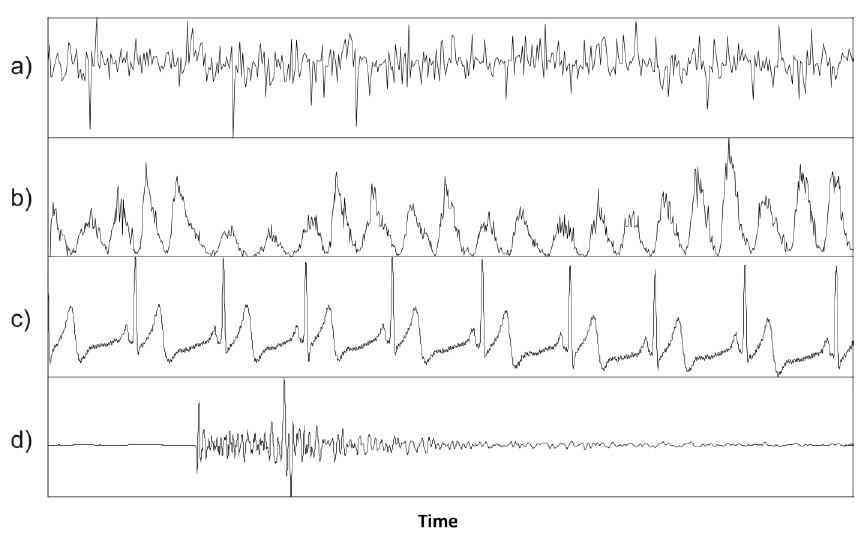
\includegraphics[scale=0.7]{timeSeries.png}\\
\vspace*{10pt}
\footnotesize{\textbf{Figura 1.} Ejemplo de datos de series temporales relacionados con: \textbf{a)} Monz\'on, \textbf{b)} Manchas Solares, \textbf{c)} Electrocardiograma, \textbf{d)} Se\~nales S\'ismicas.}\\ \textbf{Fuente:} \cite{concepts}.
\end{center}
La representaci\'on matem\'atica m\'as frecuente de una serie temporal multivariable, puede definirse de la siguiente manera:\\
$y_1, y_2,...,y_N; (y_t)^N t=1; (y_t: t=1,...,N)$, donde $y_t \equiv [y_t1, y_t2,...,y_tM]' (m \geq 2)$ es la observaci\'on $n^0$ $t(1 \leq t \leq N)$ de la serie y N es el n\'umero de observaciones que conforman la serie completa.\\
Las observaciones pueden ser almacenas en una matriz $Y$ de orden $N X M$:\\
\begin{equation}
Y \equiv \kbordermatrix{
				 & {    } \\	
				 & {y'_1} \\
				 & {y'_2} \\
				 & {.}    \\
				 & {.}    \\
 				 & {.}    \\
 				 & {y'_N} \\
		} \equiv
\kbordermatrix{
				 & {    }  & {    }   & {     } & {     } & {     } & {     }\\	
				 & {y'_{11}} & {y'_{12}}  & {  .  } & {  .  } & {  .  } & { y_{1M}}\\	
				 & {y'_{21}} & {y'_{22}}  & {  .  } & {  .  } & {  .  } & { y_{2M}}\\	
				 & {.}     & {.} &  &  &  & {.} \\
				 & {.}     & {.} &  &  &  & {.} \\
 				 & {.}     & {.} &  &  &  & {.} \\
 				 & {y'_{N1}} & {y'_{N2}} & {.} & {.} & {.} & {y_{NM}}  \\
}
\end{equation}\\
donde $y_{tj}$ es la observaci\'on $n^0$ $t(1 \leq t \leq N)$ sobre la caracter\'istica o variable $n^0$ $j(1 \leq t \leq N)$, que es la misma en todo momento $t$ \cite{concepts}.
\subsection{Aplicaci\'on y An\'alisis de Series Temporales}
La medici\'on y el seguimiento del comportamiento de alg\'un fen\'omeno o los datos espec\'ificos de alguna actividad en el tiempo, pueden producir informaci\'on muy relevante. Es informaci\'on de primera mano, que puede ser utilizada para comprender mejor aquello que ha venido ocurriendo, monitorear el estado actual para explicar la relaci\'on causal o la estructura subyacente que producen los datos observados, y finalmente, permite realizar predicciones o pron\'osticos que podr\'ian proveer un control anticipado sobre el fen\'omeno que se est\'a estudiando.\\
Muchas series temporales tienen una tendencia creciente, por ejemplo, el n\'umero de autom\'oviles en uso en casi todos los pa\'ises durante los \'ultimos cincuenta a\~nos, o decreciente como el n\'umero de personas que trabajan en la agricultura; otras sin embargo, no tienen tendencia y son estacionarias, por ejemplo, la luminosidad a horas sucesivas, que var\'ia c\'iclicamente a lo largo de las 24 horas del d\'ia.\\
Por otra parte, existe una amplia gama de aplicaciones, en campos como la medicina, el an\'alisis bursatil, la meteorolog\'ia, la geof\'isica, la astrof\'isica, entre muchas otras disciplinas, cuyas observaciones pueden ser representadas como series de tiempo. Dichas observaciones, pueden ser exploradas y analizadas mediante el uso de t\'ecnicas de \textit{mineria de datos}, por ejemplo, a trav\'es del descubrimiento de patrones y el agrupamiento (clustering), t\'ecnicas  de clasificaci\'on, el descubrimiento de reglas y el resumen o la abstracci\'on de los datos.\\
Como se explicar\'a m\'as adelante durante el desarrollo de este documento, la propuesta de investigaci\'on se enfoca principalmente en la mejora de dos algoritmos utilizados en el descubrimiento de reglas significativas en series temporales.
\subsection{Grandes Retos Sobre la Miner\'ia de Series Temporales}
El an\'alisis y el descubrimiento de patrones sobre series temporales, por definici\'on, presenta una serie de retos y complicaciones que deben abordarse tales como: la super multidimensional, la presencia de grandes cantidades de datos que muchas veces resultan innecesarios o poco \'utiles durante el an\'alisis, la sensibilidad al ruido o a la presencia de valores at\'ipicos y el dinamismo durante la transmici\'on de datos o \textit{\enquote{data streaming}}, debido a que requiere un procesamiento de datos temporales a una gran velocidad, fluctuando const\'antemente y potencialmente infinitos \cite{main}.\\
Por otra parte, \textit{\textbf{el c\'alculo de la similitud}} durante la comparaci\'on de dos o m\'as series temporales es considerado un desaf\'io a\'un mucho m\'as crucial en la miner\'ia de series temporales, especialmente cuando se ha realizado previamente una reducci\'on de la dimensionalidad, de la escala o la amplitud a trav\'es del tiempo. La carencia de un alineamiento oportuno sobre el eje tiempo o la amplitud, durante el c\'alculo de la similitud entre dos o m\'as series temporales, es un problema serio porque tiene un impacto directo sobre el resultado de la comparaci\'on. \cite{concepts}.\\
El c\'alculo de la similitud, es indispensable en la identificaci\'on de segmentos repetitivos contenidos en la serie de tiempo. Estos patrones se conocen como \textit{\textbf{\enquote{motivos}}} o \textit{\textbf{\enquote{motifs}}}, los cuales, pueden definirse como patrones o \textit{ocurrencias frecuentes de un subconjunto de la serie temporal} \cite{main}.\\
Los motifs pueden considerarse conocimiento puro o significativo, cuando como producto del minado de la serie temporal, se puede utilizar el \textit{motif} para explicar e incluso predecir, con una probabilidad, un fen\'omeno en el corto o el largo plazo.
\subsection{Medidas de Similitud}
 We can identify motifs (i.e., frequently occurring
sequential patterns) and build index or hashing mechanisms for an efficient search
based on such motifs









